 \documentclass{beamer}
\mode<presentation> {
\usetheme{PaloAlto}
\usecolortheme{dove}
\setbeamertemplate{footline}[page number] 
}

\usepackage{polski}
\usepackage[utf8]{inputenc}
\usepackage{neuralnetwork}
\usepackage{adjustbox}
\usepackage{xcolor}
\usepackage{minted}

\setbeamertemplate{caption}[numbered]

\defbeamertemplate{description item}{align left}{\insertdescriptionitem\hfill}
% \beamertemplatenavigationsymbolsempty
\setbeamertemplate{description item}[align left]
%\usepackage{subcaption}
%----------------------------------------------------------------------------------------
%	TITLE PAGE
%----------------------------------------------------------------------------------------
\title[Cykl życia obiektów]{Inicjalizacja i niszczenie obiektów w wybranym języku programowania.} % The short title appears at the bottom of every slide, the full title is only on the title page

\author{Patryk Lisik} % Your name
\institute[] % Your institution as it will appear on the bottom of every slide, may be shorthand to save space
{
 Uniwersytet Łódzki \\ % Your institution for the title page
}

\date{2023/24} % Date, can be changed to a custom date

\begin{document}

\begin{frame}
\titlepage
% Print the title page as the first slide
\end{frame}

\begin{frame}{Agenda}
    \begin{itemize}
        \item Pojęcia
        \item  Inicjalizacja w językach systemowych. 
            \begin{itemize}
                \item Stos (stack)
                \item Sterta (heap)
                \item Problem fragmentacji
                \item Alokacja pamięci
            \end{itemize}
        \item Inicjalizacja w językach obiektowych
        \item Bezpieczeństwo pamięci w językach bez GC
            \begin{itemize}
                \item Zliczanie referencji(shared\_prt)
                \item Przekazywanie własności(unique\_ptr)
            \end{itemize}
        \item Problem cyklicznych referencji
        \item Garbage collectory 
            \begin{itemize}
                    \item Taksonomia
                    \item Działanie Mark/Sweep/Compact
                
            \end{itemize}

    \end{itemize}
\end{frame}

%----------------------------------------------------------------------------------
\section{Pojęcia}

\begin{frame}[containsverbatim]{Co to typ?}
    \begin{block}{Typ}
        Dane i zbiór operacji, które można na nich wykonać \cite{IBM-What-is-type}.
    \end{block}
    \begin{figure}
        \centering
        \inputminted{cpp}{./LineFunc.cpp}
    \caption{Przykład własnego typu w C++}
        \label{fig:cpp-operator-oveerload}
    \end{figure}

\end{frame}


\begin{frame}[containsverbatim]{Co to obiekt?}

    \begin{block}{Obiekt}
        Ukonkretnienie typu w postaci zaalokowanej pamięci. 
    \end{block}

    \begin{block}{}
    \begin{figure}
        \centering
        \inputminted{cpp}{./cpp_object.cpp}
        \label{fig:cpp-obj-on-stack}
    \end{figure}

    \end{block}
    
\end{frame}

\begin{frame}{Rola systemu operacyjnego w przydziale pamięci}
    \begin{columns}
        \begin{column}{0.58\textwidth} 
            \begin{figure}
                \centering
                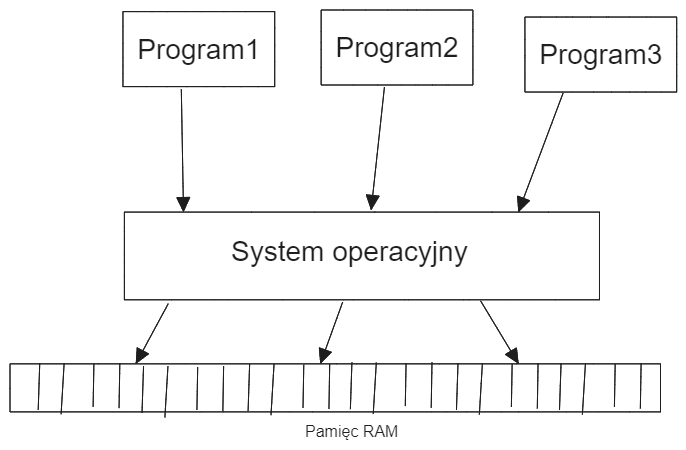
\includegraphics[width=7cm]{./os_in_memory_alloc.png}
                \caption{Układ pamięci programu}
                \label{img:os_in_memory_alloc}
            \end{figure}
        \end{column}
        \begin{column}{0.4\textwidth} 
            \begin{itemize}
                    \item Program/Process ma dostęp tylko do pamięci przydzielonej przez OS.
                    \item Odczyt z nie dozwolonej pamięci kończy się wyjątkiem segmentation fault core dumped
            \end{itemize}
        \end{column}
\end{columns}


\end{frame}


\begin{frame}[containsverbatim]{Pamięć programu}

\begin{columns}
    \begin{column}{0.5\textwidth} 
        \begin{figure}
        \centering
        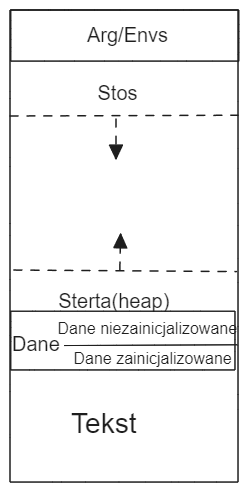
\includegraphics[width=2cm]{memory_layout.png}
        \caption{Układ pamięci programu}
        \label{img:memory_layout}
        \end{figure}
    \end{column}
        \begin{column}{0.5\textwidth} 
        \begin{block}{}
            \begin{description}
                \item [Argumenty] *argc, zmienne środowiskowe
                \item [Stos] Zmienne lokalne programu. ok 1mb
                \item [Sterta] Dane alokowane dynamicznie
                \item [Dane] Zmienne globalne, vtable, 
                \item [Tekst] Kod programu
            \end{description}
        \end{block}
    \end{column}
\end{columns}

\end{frame}


\section{Inicjalizacja w językach systemowych}

%----------------------------------------------------------------------------------------
%     class LineFucntion {
%         public:
%             double a, b; //dane

%         // operajca
%         double operator()(double x) const{ 
%             return a * x + b;
%         }
%     };


% int main(){
%     LineFucntion func{4.5, 2.1};
%     double d = func(7.2);
%     return 0;
% }

%----------------------------------------------------------------------------------------

\begin{frame}[containsverbatim]{Alokacja na stosie}
    \begin{columns}
        \begin{column}{0.3\textwidth} 
            \inputminted{cpp}{stack_alloc.cpp}
        \end{column}
        \begin{column}{0.65\textwidth} 
            \begin{description}
                \item[Szybkość] Kolejna zmienna jest zawsze alokowana na wskaźniku stosu +1
                \item[Rozmiar] Rozmiar stosu jest stały. 
                    Przy jego przekroczeniu występuje wyjątek stack overflow.
                \item[Dane] Rozmiar danych przechowywanych na stosie musi być znany w czasie kompilacji.
            \end{description}
        \end{column}
    \end{columns}
\end{frame}

\begin{frame}{Dynamiczna alokacja na stosie?}
    \begin{columns}
        \begin{column}{0.3\textwidth} 
            \inputminted{cpp}{stack_alloc.cpp}
        \end{column}
        \begin{column}{0.65\textwidth} 
        \begin{figure}
        \centering
        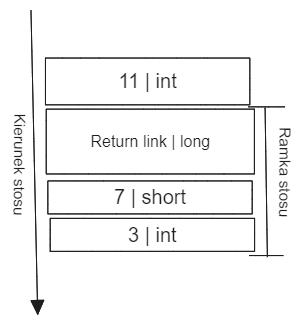
\includegraphics[width=5cm]{stack_of_foo.png}
        \end{figure}
        \end{column}
    \end{columns}
    \begin{block}{}
        Dynamiczna alokacja na stosie jest niemożliwa, ponieważ elementy nadpisywały by swoje wartości. 
    \end{block}
\end{frame}
    
    

\begin{frame}{Alokacja na stercie}
    
    \begin{columns}
        \begin{column}{0.3\textwidth} 
            \inputminted{cpp}{stack_alloc.cpp}
        \end{column}
        \begin{column}{0.65\textwidth} 
            \begin{description}
                \item[Szybkość] Kolejna zmienna jest zawsze alokowana na wskaźniku stosu +1
                \item[Ograniczony rozmiar] Rozmiar stosu jest stały. 
                    Przy jego przekroczeniu występuje wyjątek stack overflow.
            \end{description}
        \end{column}
    \end{columns}
\end{frame} 

\begin{frame}{Działanie malloc/new}


\end{frame}
% \begin{frame}[containsverbatim]{Typy alokacji}
%     \begin{figure}
%         \centering
%         \tiny
%     \begin{minted}{cpp}
%             int main(){
%                 LineFucntion func{4.5, 2.1};
%                 double d = func(7.2);
%                 puts("In between");
%                 return 0;
%             }
%     \end{minted}
%         \label{fig:cpp-stack-allocation}
%         \caption{Alokacja na stosie}
%     \end{figure}
    
%     \begin{figure}
%         \centering
%         \tiny
%     \begin{minted}{cpp}
%             int main(){
%                 LineFucntion* func = new LineFucntion(4.5, 2.1);
%                 double d = (*func)(7.2);
%                 puts("In between");
%                 delete func;
%                 return 0;
%             }
%     \end{minted}
%         \label{fig:cpp-heap-allocation}
%         \caption{Alokacja na stercie.}
%     \end{figure}
% \end{frame}

% \begin{frame}[containsverbatim]{Konstruktor}
%     \begin{figure}
%         \centering
%         \tiny
%     \begin{minted}{cpp}
%     #include <cstdio>
%     #include <algorithm>
%     class LineFucntion {
%         public:
%             double a, b;
%             //konstruktor
%             LineFucntion(double a , double b){ 
%                 puts("Constructor");
%                 this->a=a;
%                 this->b=b;
%             }

%             // kontruktor kopiujący 
%             LineFucntion(LineFucntion const & lf){
%                  puts("Copy constuctor");
%             }

%             //destruktor
%             ~LineFucntion(){
%                 puts("Destructor");
%             }
%         double operator()(double x) const{ return a * x + b;}
%     };


%     \end{minted}
%         \label{fig:cpp-constructor}
%         \caption{Jawnie zdefniowany konstruktor w C++. Zgodnie z zasadą 0/3/5.}
%     \end{figure}
    
% \end{frame}


\begin{frame}{Alokacja pamięci}
    \begin{block}{Alokacja pamięci}
        Alokacja pamięci to rezerwacja przez system operacyjny pamięci dla procesu\cite{mmap-linux_man, virtual-alloc}.
        
        \textit{(Nie rozpatrujmy sytuacji gdy nie ma systemu operacyjnego)}
    \end{block}
    \begin{block}{POSIX}
        W systemach zgodnych z POSIX alokacja pamięci odbywa się poprzez  `mmap()` \cite{mmap-linux_man}.
    \end{block}

    \begin{block}{Windows}
        W systemach Windows alokacja pamięci odbywa się poprzez VirtualAlloc[memoryapi.h] \cite{virtual-alloc}.
    \end{block}
\end{frame}

\begin{frame}[containsverbatim]{Bezpieczeństwo pamięci w językach bez GC}
\begin{minted}{cpp}
class ChildFucntion : public LineFucntion { 
    public:
ChildFucntion(double a, double b): LineFunction(a,b){
    puts("Child");}
    
ChildFucntion(ChildFucntion const & cf{
    puts("Child copy constuctor");
    }
~CholdFucntion(){puts("Child destructor");}
    }
\end{minted}
\begin{block}{}
    Najpierw wywoływany jest konstruktor rodzica.
\end{block}
\end{frame}
%----------------------------------------------------------------------------------------
\section{Automatyczne zarządzanie pamięcią w C++}

\begin{frame}{Zliczanie referencji}
    \begin{block}{}
        std:shared\_ptr składa się z licznika referencji i właściwego wskaźnika. 
        Podczas kopi licznik referencji jest zwiększany, a podczas wywołania destruktora zmniejszany. 
        Przy wywołaniu ostatniego destruktora pamięć jest zwlaniana \cite{cpp-shared-ptr}. 
    \end{block}
\end{frame}


\begin{frame}{Uniqe\_ptr}
    \begin{block}{Własność w programowaniu}
        Własność określa kto jest odpowiedzialny za zwolnienie pamięci \cite{rust-ownership, cpp-unique-ptr}.
    \end{block}

    \begin{block}{}
        std::move informuje kompilator o możliwości przeniesienie zasobów już istniejącego obiektu.
    \end{block}
\end{frame}

%----------------------------------------------------------------------------------------

%----------------------------------------------------------------------------------------
\begin{frame}{Problem cyklicznych referencji}
    \begin{figure}
        \centering
        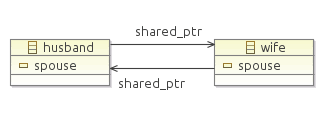
\includegraphics[width=7cm]{cyclic_ref.png}
        \caption{Problem cyklicznych referencji gdzie pamięć nigdy nie jest zwalniana. Źródło: \cite{weak-ptr-vs-magazine}}
        \label{fig:enter-label}
    \end{figure}

\begin{block}{std::weak\_ptr}
    Rozwiązaniem problemu cyklicznych referencji jest referencja słaba(std::weak\_ptr) która nie powoduje inkrementacji licznika referencji. Nie gwarantuje one że obiekt nie został już usunięty \cite{weak-ptr-vs-magazine, cpp-weak-ptr}. 
\end{block}
\end{frame}

\section{Odśmiecanie  Garbage Collctor}

\begin{frame}{Oznacz i zmieć (ang. \textit{mark and sweep})}
    \begin{block}{Faza mark}
        Przeszukujemy "w głąb" graf obiektów i oznaczamy każdy obiekt do którego dotarliśmy \cite{mark-and-sweep}. 
    \end{block}
    \begin{block}{Faza sweep}
        Usuwamy obiekty nieoznaczone.
    \end{block}
        \begin{block}{Faza compact(Opcjonalna)}
        Obiekty przesuwane są blisko siebie w pamięci.
    \end{block}

    \begin{block}{Krytyka}
    \begin{itemize}
        \item Jest to bardzo wolny algorytm, który wymaga zatrzymania przetwarzania do działania (ang. \textit{stop the world GC}).
        \item  Bez fazy compact powoduje dużą fragmentację pamięci. 
    \end{itemize}
    \end{block}
\end{frame}

\begin{frame}{Inne rodzaje odśmiecaczy/garbage collectorów}
\begin{block}{}
Generacyjny \\
Trzykolorowy  \\
Arenowy
\end{block}


\end{frame}

\begin{frame}[allowframebreaks]{Literatura}
\bibliographystyle{ieeetr}
\bibliography{refs} 
\end{frame}


\end{document}
